\documentclass[colorlinks]{beamer}

\usepackage[utf8]{inputenc}
\usepackage{fancybox,fancyvrb}
\usepackage{environ}
\usepackage{tikz}

\beamertemplatenavigationsymbolsempty
\setbeamertemplate{footline}[frame number]

\newcommand{\ds}{\displaystyle}


\title{2.1 Solution Curves \\ (direction fields and phase portraits)}

\subtitle{a lecture for MATH F302 Differential Equations}

\author{Ed Bueler, Dept.~of Mathematics and Statistics, UAF}

\date{Fall 2023}

\usetheme{Pittsburgh}


\begin{document}

\setbeamertemplate{itemize item}{$\bullet$}
\setbeamertemplate{itemize subitem}{$\circ$}


\begin{frame}
\titlepage

\centerline{\tiny for textbook: \, D. Zill, \emph{A First Course in Differential Equations with Modeling Applications}, 11th ed.}
%\color{green!40!blue}
\end{frame}


\begin{frame}{meaning of a differential equation}

\begin{itemize}
\item let us start over on the meaning of a differential equation (DE)
\item for the DE
    $$\frac{dy}{dx} = f(x,y)$$

\vspace{-2mm}
    \begin{enumerate}
    \item the left side is the \emph{slope} of the solution $y(x)$
    \item given a point $(x,y)$, the right side computes a number $f(x,y)$
    \end{enumerate}
\item thus a first-order DE says:
    $$\begin{matrix}
    \text{the slope of the} \\
    \text{solution } y(x) 
    \end{matrix} \quad \stackrel{\text{equals}}{=} \quad
    \begin{matrix}
    \text{a known function of} \\
    \text{the location } (x,y)
    \end{matrix}$$
\end{itemize}
\end{frame}


\begin{frame}{picturing a DE}

\begin{itemize}
\item the first-order DE \quad $\ds \frac{dy}{dx} = f(x,y)$ \quad says:
    $$\boxed{\begin{matrix}
    \text{the slope of the} \\
    \text{solution } y(x) 
    \end{matrix} \quad \text{equals} \quad
    \begin{matrix}
    \text{a known function of} \\
    \text{the location } (x,y)
    \end{matrix}}$$

\item this means that

\centerline{\alert{we can \emph{draw} a picture of the DE itself}}

by drawing the slope $m=\frac{dy}{dx}$ at each point $(x,y)$

\item we can do this whether or not we can do the calculus/algebra to find a solution formula $y(x)$
\end{itemize}
\end{frame}


\begin{frame}{direction field}

\begin{itemize}
\item from the first-order DE $\ds \frac{dy}{dx} = f(x,y)$ we can create a \emph{direction field} or \emph{slope field}:
    \begin{enumerate}
    \item generate a grid of point in the $x$,$y$ plane
    \item for each point, draw a short line segment with the slope given by $f(x,y)$ at that point
    \end{enumerate}

\bigskip
\item \begin{minipage}[t]{0.32\textwidth}
\emph{Example.}  By hand, draw a direction field:
$$\frac{dy}{dx} = x-y$$
on the square

$-3 \le x \le 3$,

$-3 \le y \le 3$
\end{minipage} 

\vspace{20mm}
\end{itemize}
\end{frame}


\begin{frame}{computers are useful}

\begin{itemize}
\item I \emph{happily} acknowledge that this is a job for a computer!
    \begin{itemize}
    \item see the \href{https://bueler.github.io/math302/codes.html}{Codes tab} at the public site
    \item I will use a Python function \texttt{dirfield()}
    \end{itemize}

\medskip
\item \emph{Example.}  Use a computer to draw a direction field for
$\frac{dy}{dx} = x-y$ on the square $-3 \le x \le 3, -3 \le y \le 3$

\bigskip
\emph{Solution}:

\vspace{-3mm}
\hfill 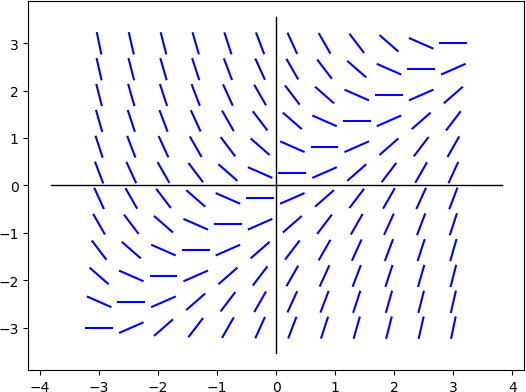
\includegraphics[width=0.5\textwidth]{figs/example-field} \phantom{as dfjadl dsf}

\medskip
\scriptsize
\texttt{def f(x,y):  return x - y}  \hfill $\longleftarrow$ \emph{Python code}

\texttt{dirfield(f,[-3,3,-3,3],mx=12,my=12)}
\end{itemize}
\end{frame}


\begin{frame}{picturing IVPs}

\begin{itemize}
\item recall that we are often solving initial value problems (IVPs)
\item \emph{next main idea}:  one can \emph{see} the solution to an ODE IVP by plotting the initial point in the plane and then following the direction field from that point

\bigskip
\item \begin{minipage}[t]{0.32\textwidth} \small
\emph{Example.}  Use the direction field for
$\frac{dy}{dx} = x-y$ to sketch the solution $y(x)$ of
    $$\frac{dy}{dx} = x-y, \, y(0)=2$$

    \begin{itemize}
    \item soon: methods in \S 2.3 will give a formula for $y(x)$
    \end{itemize}
\end{minipage}

\vspace{-45mm}
\hfill 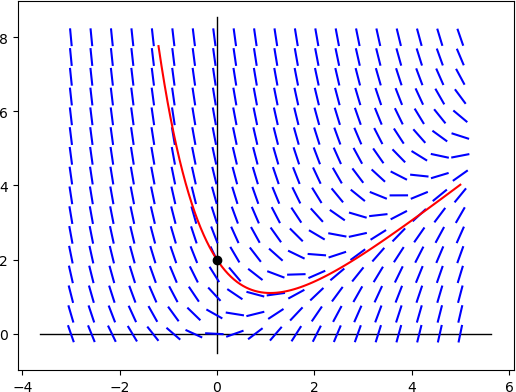
\includegraphics[width=0.55\textwidth]{figs/example-field-solution}
\end{itemize}
\end{frame}


\begin{frame}{exercise 9 in \S 2.1}

\begin{columns}
\begin{column}{0.45\textwidth}
\small
\noindent \textbf{9}.  \emph{Use computer software to obtain a direction field for the given differential equation.  By hand, sketch an approximate solution curve passing through each of the given points.}

$$\frac{dy}{dx} = 0.2 x^2 + y$$

\noindent \textbf{(a)} \quad $y(0)=\tfrac{1}{2}$

\noindent \textbf{(b)} \quad $y(2)=-1$

\vspace{15mm}

\scriptsize
\texttt{def f(x,y):  return 0.2*x**2 + y}

\texttt{dirfield(f,[-2,5,-3,3],mx=12,my=12)}
\end{column}
\begin{column}{0.55\textwidth}

\hspace{-10mm} 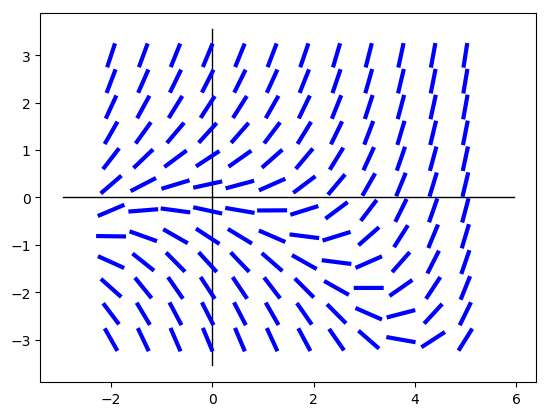
\includegraphics[width=1.15\textwidth]{figs/exercise-9-2-1}
\end{column}
\end{columns}
\end{frame}


\begin{frame}{two topics in \S 2.1}

\begin{itemize}
\item there are two equally-important topics in \S 2.1:
    \begin{itemize}
    \item \alert{direction fields} for 1st-order DEs
    \item \alert{autonomous} 1st-order DEs, and their \alert{phase portraits}
    \end{itemize}
\item both topics are about \emph{picturing DEs}

\bigskip
\item next: ``autonomous'' describes a special case where we can draw a simpler picture
\end{itemize}
\end{frame}


\begin{frame}{autonomous first-order DEs}

\begin{itemize}
\item \emph{definition}. a first-order differential equation is \emph{autonomous} if the function does not depend on the independent variable:
    $$\frac{dy}{dx} = f(y)$$

\medskip
    \begin{itemize}
    \item ``autonomous'' means ``independent of control''
    \item \dots above DE is not directly controlled by input variable $x$
    \item note that the \emph{solution} $y(x)$ is still a function of $x$
    \end{itemize}

\bigskip
\item a big idea: fundamental laws of nature, in which the independent variable is the time $t$, are autonomous DEs
\end{itemize}
\end{frame}


\begin{frame}{autonomous first-order DEs}

\begin{itemize}
\item \emph{definition}. a first-order differential equation is \emph{autonomous} if the function does not depend on the independent variable:
    $$\frac{dy}{dx} = f(y)$$

\bigskip
\item Example.
    $$\frac{dy}{dx} = \sqrt{\sin(y)} \quad \text{is autonomous}$$
\item Example.
    $$\frac{dy}{dx} = x-y \quad \text{is \emph{not} autonomous}$$
\end{itemize}
\end{frame}


\begin{frame}{classification of first-order DEs}

\begin{itemize}
\item we will see that ``autonomous'' also means ``easier to visualize,'' but \emph{not} necessarily easier to solve
\item using definitions from sections 1.1 and 2.1 we already have a \emph{classification} of first-order DEs:

\bigskip
\begin{center}
\begin{tabular}{c|c|c}
 & autonomous & nonautonomous \\ \hline
linear \Large\strut & $y' + c\, y = d$ & $y' + P(x) y = g(x)$ \\ \hline
nonlinear \Large\strut & $y' = f(y)$ & $y'=f(x,y)$
\end{tabular}
\end{center}

\bigskip
    \begin{itemize}
    \item[$\circ$] all of these can be written as $y'=f(x,y)$, right?
    \end{itemize}
\end{itemize}
\end{frame}


\begin{frame}{picturing autonomous DEs}

\begin{itemize}
\item the direction field of an autonomous DE has redundancies
    \begin{itemize}
    \item[$\circ$] since $f(y)$ only depends on $y$, the slope is the same for all $x$ values
    \end{itemize}

\medskip
\item \begin{minipage}[t]{0.35\textwidth} \small
Example.  Consider
$$\frac{dy}{dx} = \cos(2y)$$
Use a computer to draw the direction field for $x \in [-3,3]$ and $y\in [-\pi,\pi]$.  Then draw the phase portrait.
\end{minipage}

\vspace{-35mm}
\hfill 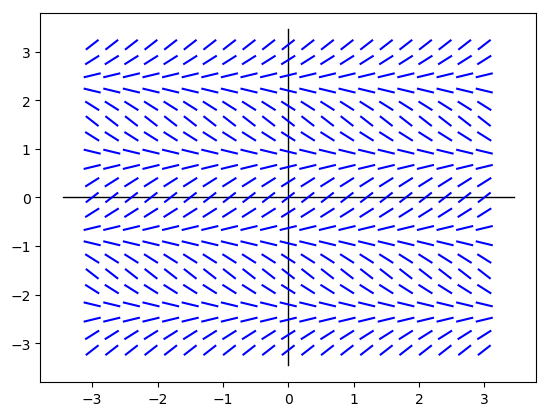
\includegraphics[width=0.5\textwidth]{figs/autonomous-cos} \phantom{ld}
% import numpy as np
% def f(x,y):  return np.cos(2*y)
% df.dirfield(f,[-3,3,-np.pi,np.pi],mx=21,my=21,slopeslinewidth=1.5)

\bigskip
\item the one-dimensional \emph{phase portrait} is a simplified form of the direction field
    \begin{itemize}
    \item a.k.a.~\emph{phase line}
    \end{itemize}

\end{itemize}
\end{frame}


\begin{frame}{critical points of autonomous DEs}

\begin{itemize}
\item consider an autonomous first-order DE: \quad $\frac{dy}{dx} = f(y)$
\item a value $y=c$ is called a \emph{critical point} if $f(c)=0$
    \begin{itemize}
    \item a.k.a.~\emph{equilibrium point} or \emph{stationary point}
    \end{itemize}

\medskip
\item if $y=c$ is a critical point then $y(x)=c$ is a solution!

\medskip
\item Example.  $y=\frac{\pi}{4}$ is a critical point \emph{and a solution} of
    $$\frac{dy}{dx} = \cos(2y)$$

\vspace{5mm}
\end{itemize}
\end{frame}


\begin{frame}{phase portrait example}

\begin{itemize}
\small
\item \begin{minipage}[t]{0.4\textwidth}
Example.  By hand, sketch the phase portrait of
   $$\frac{dz}{dt} = z^2 + z^3$$
and show all critical points.  Then sketch the graph of solutions to the ODE IVP with the following initial values.
    \begin{itemize}
    \item[\color{black} \textbf{(a)}] $z(0)=1$
    \item[\color{black} \textbf{(b)}] $z(0)=-1/2$
    \item[\color{black} \textbf{(c)}] $z(0)=-1$
    \item[\color{black} \textbf{(c)}] $z(0)=-2$
    \end{itemize}
\end{minipage}
\end{itemize}
\end{frame}


\begin{frame}{to draw a phase portrait of an autonomous equation}

for:
    $$\frac{dy}{dx}=f(y)$$
summary:
\begin{itemize}
    \item draw the $y$-axis vertically
    \item solve $f(y)=0$ for the critical points, and mark them
    \item between critical points, evaluate the sign of $f(y)$
    \item draw an up or down arrow accordingly
\end{itemize}

\bigskip
\emph{easy}!
\end{frame}


\begin{frame}{classifying critical points}

\begin{itemize}
\item a critical point $y=c$ of an autonomous differential equation $\ds \frac{dy}{dx} = f(y)$ is
    \begin{itemize}
    \item \emph{attracting} or \emph{asymptotically stable} if
\begin{equation}
        \lim_{x \to \infty} y(x) = c   \tag{$\ast$}
\end{equation}
    for all initial points $(x_0,y_0)$ where $y_0$ is close to $c$,
    \item \emph{semi-stable} if ($\ast$) only happens for $y_0$ on one side of $c$, and
    \item \emph{repelling} or \emph{asymptotically unstable} otherwise
    \end{itemize}
\end{itemize}
\end{frame}


\begin{frame}{example 2}

\small
\begin{minipage}[t]{0.5\textwidth}
\begin{itemize}
\item Example. Find and classify the critical points of
   $$\frac{dy}{dx} = \cos(2y)$$

\vspace{40mm}
\end{itemize}
\end{minipage}
\end{frame}


\begin{frame}{example 3}

\small
\begin{minipage}[t]{0.5\textwidth}
\begin{itemize}
\item Example. Find and classify the critical points of
   $$\frac{dz}{dt} = z^2 + z^3$$

\vspace{40mm}
\end{itemize}
\end{minipage}
\end{frame}


\begin{frame}{exercise 27 in \S 2.1}

\small
\begin{minipage}[t]{0.45\textwidth}
\noindent \textbf{27}.  \emph{Find the critical points and phase portrait.  Classify each critical point as asymptotically stable, unstable, or semi-stable.  By hand, sketch typical solution curves in the regions in the $xy$--plane determined by the graphs of the equilibrium solutions.}

$$\frac{dy}{dx} = y \ln(y+2)$$
\end{minipage}

\vspace{20mm}
\end{frame}


\begin{frame}{exercise 40 in \S 2.1}

\small
\begin{minipage}[t]{0.5\textwidth}
\noindent \textbf{40}.  \emph{The autonomous differential equation}

\vspace{-2mm}
$$m \frac{dv}{dt} = m g - k v,$$
\emph{where $k$ is a positive constant and $g$ is the acceleration due to gravity, is a model for the velocity $v$ of a body of mass $m$ that is falling under gravity.  The term $-kv$, which is air resistance, implies that the velocity will not increase without bound as $t$ increases.  Use a phase portrait to find the limiting, or \emph{terminal} velocity of the body.}
\end{minipage}

\vspace{10mm}
\end{frame}


\begin{frame}{looking ahead: next two sections 2.2, 2.3}

\begin{itemize}
\item the first four sections of the textbook (1.1, 1.2, 1.3, 2.1) are about the \emph{meaning} of differential equations
    \begin{itemize}
    \item such meaning \alert{is the important take-home message} from a course in differential equations!
    \end{itemize}
\item but for the next few sections we will address \alert{how to find formulas} for solutions $y(x)$
\item looking ahead to the next two sections:
\end{itemize}

\bigskip
\begin{tabular}{c|c|c}
 & autonomous & nonautonomous \\ \hline
linear \Large\strut & $y' + c\, y = d$ \alert{2.2,2.3} & $y' + P(x) y = g(x)$  \alert{2.3}\\ \hline
nonlinear \Large\strut & $y' = f(y)$ \alert{2.2} & 

\begin{minipage}{45mm}
\medskip

\small
    \begin{tabular}{c|c}
    separable & nonseparable \\ \hline
    $y'=g(x)h(y)$ \alert{2.2} & $y'=f(x,y)$
    \end{tabular}
\end{minipage}
\end{tabular}
\end{frame}


\begin{frame}{programming \dots this is not a CS class}

\begin{itemize}
\item you \emph{don't} have to know programming to do this class
\item \dots but \alert{interacting with a computer is obligatory for some homework!}
\item for such homework problems you must either embrace some coding or seek-out tools such as \href{https://www.desmos.com/}{\color{cyan} desmos} or \href{https://www.wolframalpha.com/}{\color{cyan} Wolfram alpha} which allow you to do particular computer jobs like generating direction fields
\item I will generally show a few lines of Matlab or Python when there is a computer-suitable job
\item \dots \emph{and} I'll link to some programming-free tools
\end{itemize}
\end{frame}


\begin{frame}{standard expectations}

\textbf{expectations}:  to learn this material, just listening to a lecture is \emph{not} enough
\begin{itemize}
\item please \alert{\emph{read} section 2.1 in the textbook}
    \begin{itemize}
    \item note there is a large new vocabulary in this section, namely the language of \emph{qualitative} differential equations
    \item I did not cover ``translation property'' on page 43; read that!
    \end{itemize}
\item please \alert{\emph{do} the Homework for section 2.1}
\item the visualization jobs in section 2.1 are a topic for which youtube videos etc.~can be excellent resources
\end{itemize}
\end{frame}

\end{document}

